%!TEX root = main.tex
\setcounter{chapter}{4}
\setcounter{section}{2}
\setcounter{theorem}{0}
\setcounter{equation}{0}

\lectureheader{161}{Calculus I}{Mean value theorem}{\textit{Thomas' Calculus} \thesection}

\begin{theorem}[Rolle's theorem]
Suppose that $y=f(x)$ is continuous over the closed interval $[a,b]$ and differentiable on $(a,b)$.
If $f(a)=f(b)$, then there is a $c\in (a,b)$ so that $f'(c)=0$.
\end{theorem}
\begin{center}
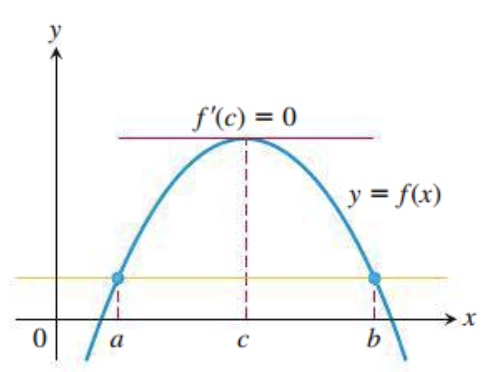
\includegraphics[width=2.5in]{img/rolles}
\end{center}

\begin{example}
Show that the equation $x^3+3x+1=0$ has \underline{exactly one} real solution.
\end{example}

\newpage

\begin{theorem}[Mean value theorem]
Suppose that $y=f(x)$ is continuous over the closed interval $[a,b]$ and differentiable on $(a,b)$.
Then there is a $c\in (a,b)$ so that
\begin{equation*}
f'(c) = \frac{f(b)-f(a)}{b-a}.
\end{equation*}
\end{theorem}
\begin{proof}\,
\begin{flushright}
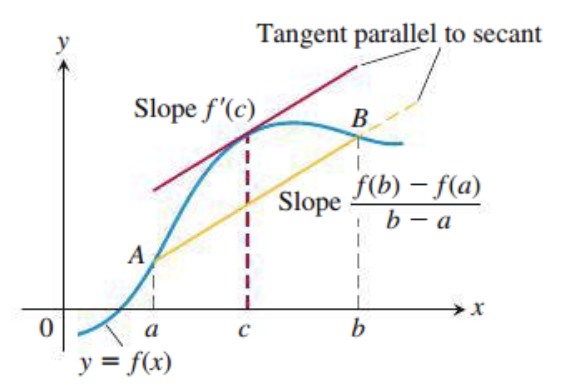
\includegraphics[width=2.5in]{img/mvt}
\end{flushright}
\vspace{4.5in}
\end{proof}
\begin{remark}
Rolle's theorem and the mean value theorem guarantee the existence of \underline{at least} one location $c\in (a,b)$ for which their respective conclusions hold.
There may be more.
\end{remark}

\newpage

\begin{example}[VASCAR]
A police officer observes a motorist pass a point $a$ on the road and then 5 seconds later pass another point $b$ at distance 500 feet away from point $a$.
What can the officer conclude?
\end{example}

\newpage

\begin{corollary}
If $f'(x)=0$ at each point in $(a,b)$, then there is a constant $C$ so that $f(x)=C$ for all $x\in (a,b)$.
\end{corollary}
\begin{proof}\,

\vspace{3in}
\end{proof}

\begin{corollary}
If $f'(x)=g'(x)$ for all $x\in (a,b)$, then there is a constant $C$ so that $f(x)=g(x)+C$ for all $x\in (a,b)$.
\end{corollary}
\begin{proof}\,

\vspace{3in}
\end{proof}

\newpage

\begin{example}
Find the function $f$ whose derivative is $\sin x$ and whose graph passes through the point $(0,2)$.
\end{example}

\newpage

\begin{theorem}[Kinematics equations] 
Suppose that an object moves along the $x$-axis with constant acceleration $a$.
If its velocity at time $t=0$ is $v_0$, then its velocity at time $t$ is
\begin{equation*}
v(t) = at + v_0.
\end{equation*}
Furthermore, if its position at time $t=0$ is $x_0$, then its position at time $t$ is
\begin{equation*}
x(t) = \frac{1}{2}at^2+v_0t + x_0.
\end{equation*}
\end{theorem}
